\section{Referee Inventory}\label{app:history}

\Cref{tab:referees} lists the referees used by the systems in
\cref{sec:road,sec:game}. The innovation game requires a reliable,
affordable referee (\cref{sub:game-boards}).





\begin{table}[htb]
  \caption{\textbf{Each domain in the main text relies on an explicit referee.}
  Rows restate the referees in \cref{sec:road,sec:game}; the last row
  \mbox{gives the} reference referee for algorithm invention.}
  \label{tab:referees}
  \centering
  \small
  \setlength{\tabcolsep}{4pt}
  \setlength{\extrarowheight}{0pt}% no row padding: the Appendix C lead-in then stays with its list
  \begin{tabularx}{\linewidth}{@{}>{\raggedright\arraybackslash}p{0.27\linewidth}>{\raggedright\arraybackslash}X>{\raggedright\arraybackslash}p{0.28\linewidth}@{}}
    \toprule
    Domain & Referee & Systems \\
    \midrule
    Board games & The rules of the game and its final score & AlphaGo Zero, AlphaZero \citep{silver2017mastering,silver2018general} \\
    Machine-learning research & A sealed test set that scores every entry & Netflix Prize, ImageNet \citep{donoho2017fifty,bennett2007netflix,russakovsky2015imagenet} \\
    Code & Unit tests; a code executor & Codex, Absolute Zero \citep{chen2021codex,zhao2025absolutezero} \\
    Matrix multiplication & The rules of TensorGame & AlphaTensor \citep{fawzi2022alphatensor} \\
    Sorting & Sorting tests & AlphaDev \citep{mankowitz2023alphadev} \\
    Mathematical constructions & Programmatic evaluators & FunSearch \citep{romeraparedes2024funsearch} \\
    Accelerator kernels & Timers & AlphaEvolve \citep{novikov2025alphaevolve} \\
    Formal proofs & The Lean proof checker & AlphaProof, STP \citep{hubert2026alphaproof,dong2025stp} \\
    RNA design & Laboratory tests of designs & EteRNA \citep{lee2014eterna} \\
    \midrule
    Algorithm invention (this paper) & Hidden-fold scores against the incumbent; promotion on strict improvement & \EZ{} (\cref{sub:game-referee,sec:method}) \\
    \bottomrule
  \end{tabularx}
\end{table}

Family allocation is separate from evaluator choice. The native audit
groups approved datasets by source identity, declared family or identical
training bytes, then assigns meta-training, meta-validation and meta-test
partitions in seeded family order. This path alone establishes neither
corpus nor checkpoint compliance with the required split.

\section{Incident Log and Audit Safeguards}\label{app:incidents}

The excluded search baseline and required safeguards appear in
\cref{sub:method-referee}. Final evaluation still needs receipts for
input closure and execution isolation:
\begin{itemize}[leftmargin=1.4em,itemsep=2pt,topsep=3pt]
  \item \textbf{Excluded test-selected search baseline.} An earlier internal
  leaderboard entry chose each dataset's best test-scored outcome from \num{63108}
  evaluations across 42 datasets. Test-fold selection biases the metric
  upward \citep{cawley2010overfitting}; the entry is \mbox{excluded from}
  all comparative claims.
  \item \textbf{Input-closure and canary checks.} Benchmark release requires
  passing receipts for an inner-fold label-poison test, a sealed canary and
  a train-only input-closure audit excluding held-out targets and derived
  statistics from both board encoding and candidate generation. The \mbox{primary evaluation record}
  in \cref{sub:results-protocol} must contain final pre-registration and receipts.
\end{itemize}

\section{Training Details}\label{app:training}

This appendix inventories the historical reference's encoder, objective
and execution requirements from \cref{sec:method}. Checkpoint
qualification remains pending; the separate adapter record appears in
\cref{sec:method-status}:
\begin{itemize}[leftmargin=1.4em,itemsep=2pt,topsep=3pt]
  \item \textbf{Board encoder blocks (\cref{sub:method-board}).} The frozen
  \num{2048}-value context $z_p = \encP(p)$ joins three blocks:
  (i)~512 pooled values from a pretrained row encoder of width 128
  across training rows by mean, population standard deviation, and 10th and 90th
  percentiles; (ii)~\num{1024} values projected from a \num{2048}-value third-party tabular
  regressor state capped at 768 context rows and 256 query
  rows (the external CPU path first subsamples to at most \num{1000} training
  rows; third-party provenance pending; restricted; redistribution prohibited); and (iii)~512 values from two
  frozen seed-17 target-summary windows. Each block is normalized before
  concatenation and clipping to $[-32,32]$. Non-finite contexts are refused. Encoding records
  report wall-clock latency from 11.7\,s to 20.8\,s across eight \mbox{reference
  encoding jobs,} within the 30\,s cap.
  \item \textbf{Comparison construction (\cref{sub:method-map,sub:method-selfplay}).}
  Lists $G_p$ require at least eight valid scored programs per problem (excluding
  stillborn draws), with
  percentile $\rho_w = 1 - \mathrm{rank}/\allowbreak{(|G_p|-1)}$ and writer $\writer$ sequence weight
  $0.05 + \rho_w^4$. The base native sampler balances families and takes
  the best program plus one draw from each of seven rank bands of the rest.
  Fresh-program replay can substitute a newly admitted candidate for
  one comparator.

  Within-comparison pairs use corpus context and comparison index;
  Python ranking helpers group by dataset identifier. Native pairing skips
  non-finite targets and exact ties, $\kappa_w=\kappa_u$, without an exclusion margin
  or logit rescaling. Training refuses non-finite supervision before loss
  formation. \mbox{\Cref{eq:writerLoss,eq:mapLoss}} give list-level losses.
  \item \textbf{Sequence supervision (\cref{eq:writerLoss}).} The native decoder
  prepends the projected context token before \texttt{BOS}. The sequence
  loss leaves \texttt{BOS} unsupervised but covers following non-padding
  tokens, including the engine and regression-task header and \texttt{EOS}.
  The header stays fixed during inference. Label smoothing of 0.05 applies
  over legal tokens; losses average within each program before the
  normalized rank-weighted mean over programs. Displayed aggregate
  coefficients match the native objective; the evaluation record must still
  identify the checkpoint objective and \mbox{its configuration}.
  \item \textbf{Runtime supervision (\cref{eq:totalLoss}).}
  The auxiliary runtime term compares $\ln(1+s)$ with
  $\ln(1+\operatorname{softplus}(h))$ by Huber loss with threshold~1,
  for measured seconds \mbox{$s\geq0$ and} raw scalar head output $h$.
  \item \textbf{Ranking targets (\cref{eq:mapLoss,eq:totalLoss}).}
  Here $\kappa_w=1/(1+\mathrm{RMSE}_w/m_p)$ (\cref{eq:totalLoss}), with $m_p$
  the corpus list's median RMSE. Microbatch Bradley--Terry weights use
  $|\kappa_w-\kappa_u|$, doubled when either member is at or above the 90th percentile.
  Weights are mean-scaled and cast to float32; weighted losses average
  non-tied within-comparison pairs in the rank-local microbatch. Listwise
  losses average eligible groups; the global-batch route uses separate reductions.
  \item \textbf{Registered parameter inventory (\cref{sub:method-map}).}
  The historical reference registers \num{27796494} parameters in total (six
  decoder blocks, width 512, four attention heads, prefix context token
  and maximum length 128 tokens over the 401-token grammar).
  Each of the writer $\writer$ and ranking-map $\mapv$ token tables allocates 657 rows:
  401 grammar rows plus 256 reserved rows. The reserved rows
  are never indexed as valid input or output tokens; the tied writer
  projection is restricted to the grammar rows.

  The registered total includes zero-weight stability and loss-scale
  terms, so it measures neither learned nor exercised capacity. Approximately
  6.90 million parameters lie outside writer token generation and share no
  weights with it: game-day decoding bypasses them; native loading requires them.
  \item \textbf{Optimization notes (\cref{sub:method-selfplay}).}
  Records describe offline AdamW training (learning rate $10^{-4}$,
  weight decay $0.01$, gradient-norm clip $1.0$, global batch size \num{2048})
  on eight A100 GPUs in September 2026 over \num{10214332} scored programs from
  80 training datasets (\num{7877} lists; \num{8894} contexts). Global batch size specifies
  neither per-GPU microbatch nor accumulation settings.
  Checkpoint acceptance and held-out promotion still require receipts
  (\cref{sub:results-protocol}).
  \item \textbf{Execution sandbox and parity (\cref{sub:method-referee}).}
  Final evaluation requires seccomp and Landlock isolation, cgroup memory
  limits, disabled swap and native/emitted-code agreement within
  $10^{-9}\max(1,|\hat{y}|)$. Its evaluation record must include final-evaluator isolation and parity
  receipts.
\end{itemize}

\section{Operating-Loop Telemetry}\label{app:flywheel-telemetry}

Adapter decisions, program-incumbent events and operating clocks count
different units (\cref{app:round-throughput}). Each capture has its own
date and population, with the scope limits in \cref{sec:method-status}.

\Cref{app:latest-admissions} begins with the adapter-admission chronology.
The later historical GP diagnostics (\cref{app:historical-search})
use a separate protocol.

% Adapter admission records, ordered by their role and capture cutoff.
\subsection{Retained admission ledger and pre-decision margins}\label{app:latest-admissions}

% Figures 14 and 15 (cited in Appendices D.2 and D.3) are defined here, at the
% start of Appendix D, so both full-width figures head the next page; defined
% after their sections, they slipped a page whenever the text above grew.
\begin{figure*}[t]
  \setlength{\abovecaptionskip}{4pt}
  \centering
  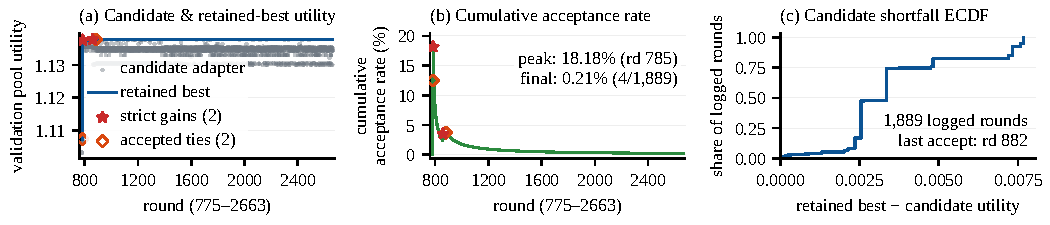
\includegraphics[width=\linewidth,height=1.50in,keepaspectratio]{figures/fig_fw_acceptance_over_rounds.pdf}
  \caption{\textbf{Cumulative adapter acceptance falls to 0.21\% across rounds 775--2663.}
  All three panels use the same \num{1889} consecutive admission evaluations (\cref{tab:admission-ledger}).
  (a) Candidate validation utility (logged scalar score; grey) and post-decision recorded best (blue), with stars at
  strict gains (rounds 785 and 859) and hollow diamonds at accepted ties (rounds 782 and 882).
  (b) Cumulative accepted share of elapsed rounds (\%), peaking at 18.18\% at round 785 and
  declining across \num{1781} subsequent rejected rounds to 0.21\% ($4/\num{1889}$).
  (c) Empirical cumulative distribution (fraction of evaluations) of recorded-best minus candidate validation utility;
  zero marks the four accepted adapter evaluations. Scope: \cref{sec:method-status}.}
  \label{fig:fw-validation}
  \label{fig:fw-acceptance-over-rounds}
  \label{fig:fw-admission-shortfall}
\end{figure*}
\begin{figure*}[!t]
  \setlength{\abovecaptionskip}{4pt}
  \centering
  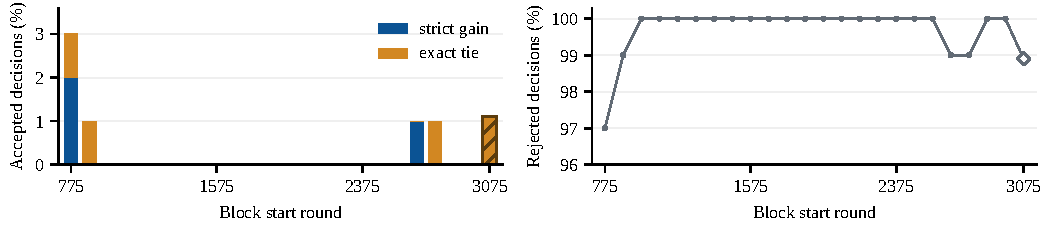
\includegraphics[width=\linewidth,height=1.55in,keepaspectratio]{figures/fig_fw_admission_block_rates.pdf}
  \caption{\textbf{Nineteen of 24 observed-round blocks record zero adapter admissions.}
  All \num{2391} complete journal decisions in rounds 775--3165, captured at 20:17 UTC
  on 1 November 2026. Blocks contain 100 consecutive observed rounds; the final
  3075--3165 block contains 91. Left: accepted strict gains (blue) and exact ties
  (orange), stacked percentages. Right: rejected decisions (\%; axis starts
  at 96\%). Each denominator is that block's observed rounds; hatching and a
  diamond mark the partial block. Totals: three strict gains, four ties and
  \num{2384} rejections. These adaptive adapter decisions are distinct from
  program-incumbent events and independent first-proposal \mbox{game-day performance. Scope: \cref{sec:method-status}.}}
  \label{fig:fw-candidate-retained-trace}
\end{figure*}

\begin{table}[!htbp]
  \caption{\textbf{The canonical admission ledger records every complete row in the prefix.}
  Strict gains and ties use unrounded candidate minus prior-best
  utility, without outcome selection. Scope: \cref{sec:method-status}.}
  \label{tab:admission-ledger}
  \centering\footnotesize\setlength{\tabcolsep}{4pt}\renewcommand{\arraystretch}{0.92}\sisetup{group-digits=integer}% full-precision logged values: roman digits and a true minus
  \begin{tabularx}{\linewidth}{@{}>{\raggedright\arraybackslash}Xl@{}}
    \toprule
    Quantity & Recorded value \\
    \midrule
    Capture cutoff (UTC) & 2026-11-02 23:00 \\
    Complete rounds & 775--3950 (\num{3176} records) \\
    Admissions / rejections & 8 / \num{3168} \\
    Strict-gain rounds & 785, 859, 2750, 3175 \\
    Exact-tie rounds & 782, 882, 2795, 3100 \\
    Final retained utility & \num{1.1389572403748425} \\
    Recorded best-round identity & 3175 \\
    New rows since prior capture & 753 (0 admitted) \\
    Rejected margins in $[-10^{-4},0)$ & 26 \\
    Rejected margins in $[-10^{-3},-10^{-4})$ & 51 \\
    Rejected margins below $-10^{-3}$ & \num{3091} \\
    Closest rejected margin & \num{-0.0000433838086485} (round 803) \\
    Median rejected margin & \num{-0.0033601045139468} \\
    \bottomrule
  \end{tabularx}
\end{table}

\Cref{tab:admission-ledger} collects the chronology, exact counts and
margin summaries for one capture. The pre-decision margin is
$\Delta_r=u_{\mathrm{cand},r}-u_{\mathrm{prev},r}$;
the default rule accepts $\Delta_r\geq0$.

\Cref{fig:fw-admission-margins} summarizes complete trailing 50-round
windows and cumulative near-tie rejections from that same record.

\subsection{Retained-best trajectory and cumulative acceptance rate}\label{app:acceptance-over-rounds}\label{app:record-windows}

\Cref{fig:fw-acceptance-over-rounds} covers \num{1889} decisions in
rounds~775--2663. From \num{1.1074}, the retained best reaches \num{1.1376} at round
785 and \num{1.1378} at 859; rounds 782 and 882 are accepted ties.
The cumulative acceptance rate reaches 18.18\% ($2/11$) at round 785,
3.70\% ($4/108$) at round 882 and 0.21\% ($4/\num{1889}$) after
\num{1781} further rejections. Each round contributes once to the
utility-shortfall distribution; rounds are not independent tasks or
distinct programs. Cross-harness comparisons require matched data,
normalization and scoring protocols.

\subsection{Admission frequency through a later cutoff}\label{app:candidate-retained-trace}

\Cref{fig:fw-candidate-retained-trace} groups the complete admission journal
from the canonical ledger's first round (\cref{tab:admission-ledger}) through
the latest complete admission matched to a retained summary. Its 24 blocks
contain 23 full blocks and one partial block; 19 have no admission, including
17 consecutive full blocks in rounds 975--2674. The 21 available summaries
(3145--3165) match the journal's scores and decisions; older rows are journal-only.
The last accepted decision, at round 3100, is an exact tie, followed by
65 rejections. Frequencies count decisions, not independent tasks, distinct
programs or a stationary admission probability. Stable log-prefix hashes bind
this separate capture. This trace retains its own capture cutoff;
the field-binding limits in \cref{sec:method-status} still apply.

\begin{figure*}[!t]
  \setlength{\abovecaptionskip}{4pt}
  \centering
  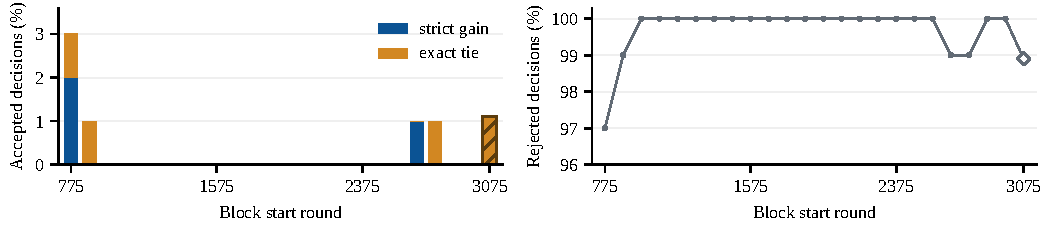
\includegraphics[width=\linewidth,height=1.55in,keepaspectratio]{figures/fig_fw_admission_block_rates.pdf}
  \caption{\textbf{Adapter admission and rejection frequencies by observed-round block.}
  All \num{2391} complete journal decisions in rounds 775--3165, captured at 20:17 UTC
  on 1 November 2026. Blocks contain 100 consecutive observed rounds; the final
  3075--3165 block contains 91. Left: accepted strict gains (blue) and exact ties
  (orange), stacked percentages. Right: rejected decisions (percent; axis starts
  at 96\%). Each denominator is that block's observed rounds; hatching and a
  diamond mark the partial block. Totals: 3 strict gains, 4 ties and
  \num{2384} rejections. These adaptive adapter decisions are distinct from
  program-incumbent events and independent first-proposal performance.
  Scope: \cref{sec:method-status}.}
  \label{fig:fw-candidate-retained-trace}
\end{figure*}

\subsection{Candidate and retained-best decisions in a recent capture}\label{app:recent-admission-trajectory}

The capture in \cref{fig:fw-recent-candidate-retained} retains the latest
500 consecutive complete admission records matched to the per-round audit.
It remains separate from earlier windows: gaps are unjoined and source
binding remains unresolved (\cref{sec:method-status}).

\begin{figure}[tbp]
  \centering
  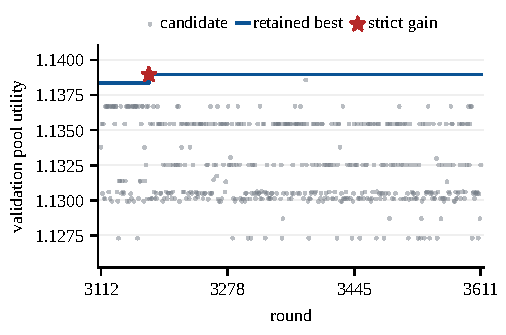
\includegraphics[width=\linewidth]{figures/fig_fw_recent_candidate_retained_trace.pdf}
  \caption{\textbf{One strict gain and 499 rejections occur in rounds \mbox{3112--3611}.}
  Rounds 3112--3611, captured at 10:25 UTC on 2 November 2026.
  Grey points show candidate utility; blue is the post-decision retained
  best (logged dimensionless utility, larger preferred). The star marks
  the one accepted strict gain, at round 3175; the other 499 decisions
  are rejections. Classification uses exact logged values, with no rounding margin.
  These are adaptive decisions on repeatedly used development contexts,
  not independent first-proposal results or evidence of writer or ranking-map lift.
  Scope: \cref{sec:method-status}.}
  \label{fig:fw-recent-candidate-retained}
\end{figure}

\FloatBarrier
\section{Rolling Adapter Admission Frequencies}\label{app:rolling-admissions}

\Cref{fig:fw-rolling-admissions} uses a separate recent capture of adapter
decisions. The earlier ledger in \cref{tab:admission-ledger} retains its
own capture and cutoff. Each trailing window contains exactly 100 observed
decisions, including accepted ties and rejected candidates. These overlapping
counts describe the logged policy on an adaptively reused development
population; the independent first-proposal comparison remains pending.

\begin{figure}[htb]
  \centering
  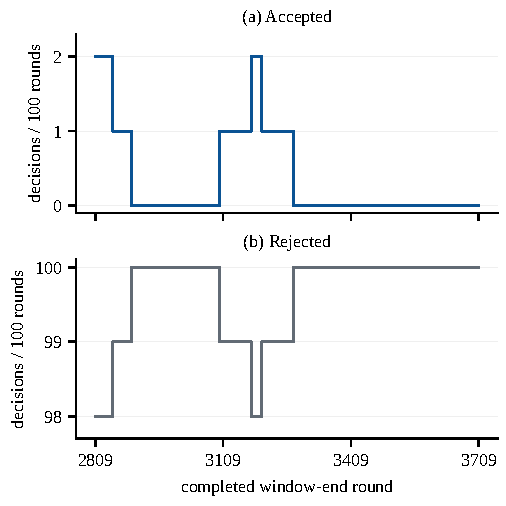
\includegraphics[width=\linewidth]{figures/fig_fw_rolling_admissions.pdf}
  \caption{\textbf{Trailing 100-round adapter acceptance and rejection counts.}
  The source window contains \num{1000} consecutive completed rounds,
  2710--3709, captured at 13:30 UTC on 2 November 2026. It records four
  admissions (two strict gains and two exact ties) and 996 rejections.
  Panels (a) and (b) show the complementary accepted and rejected counts
  in each full trailing window, plotted at its final round: 2809--3709,
  or 901 overlapping windows. The first 99 source rows supply history
  without a plotted partial window. Every accepted/rejected pair sums to
  100; one decision per 100 rounds also equals one percentage point.
  Decisions use unrounded candidate and prior-best utility.
  These are adapter admissions, distinct from training-program incumbent
  events; no uncertainty interval or independent improvement estimate is
  implied. Scope: \cref{sec:method-status}.}
  \label{fig:fw-rolling-admissions}
\end{figure}
\subsection{Recorded selection changes}\label{app:selection-changes}

The observer in \cref{fig:fw-selection-changes} refuses changed evaluation
identities, inconsistent selection counts and duplicate context identifiers
before comparing ordered program identities. It counts candidate and retained
differences from one stored reference, rather than utility changes.
The tie-admission and best-round identity rules follow
\cref{sec:method-status}.
These changes occur on reused development contexts; matched controls are
still required for \mbox{attribution to training} or proposal quality.

\begin{figure}[htbp]
  \centering
  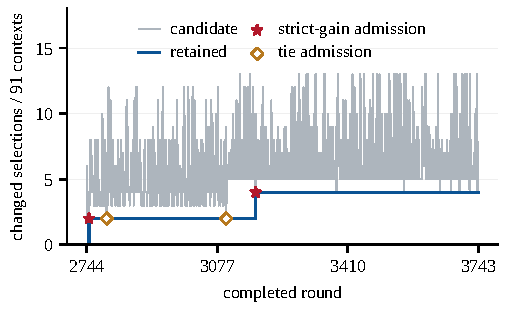
\includegraphics[width=\linewidth]{figures/fig_fw_selection_changes.pdf}
  \caption{\textbf{Retained program selections change only at admitted rounds.}
  Rounds 2744--3743, captured at 14:34 UTC on 2 November 2026.
  All \num{1000} completed records compare selections on 91 reused
  development contexts with the recorded round-882 reference.
  Grey: candidate before admission; blue: post-decision retained selections.
  Stars: two strict-gain admissions; hollow diamonds: two accepted ties;
  the other 996 decisions are rejections. These descriptive identity
  counts do not establish a training effect, writer or ranking-map benefit,
  or independent proposal quality. Scope: \cref{sec:method-status}.}
  \label{fig:fw-selection-changes}
\end{figure}


\subsection{Recorded selection changes}\label{app:selection-changes}

The observer in \cref{fig:fw-selection-changes} refuses changed evaluation
identities, inconsistent selection counts and duplicate context identifiers
before comparing ordered program identities. It counts candidate and retained
differences from one stored reference, rather than utility changes.
The tie-admission and best-round identity rules follow
\cref{sec:method-status}.
These changes occur on reused development contexts; matched controls are
still required for \mbox{attribution to training} or proposal quality.

\begin{figure}[htbp]
  \centering
  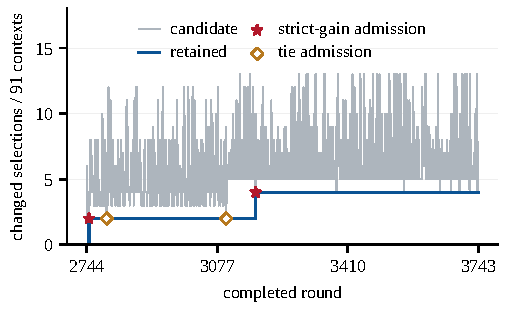
\includegraphics[width=\linewidth]{figures/fig_fw_selection_changes.pdf}
  \caption{\textbf{Retained program selections change only at admitted rounds.}
  Rounds 2744--3743, captured at 14:34 UTC on 2 November 2026.
  All \num{1000} completed records compare selections on 91 reused
  development contexts with the recorded round-882 reference.
  Grey: candidate before admission; blue: post-decision retained selections.
  Stars: two strict-gain admissions; hollow diamonds: two accepted ties;
  the other 996 decisions are rejections. These descriptive identity
  counts do not establish a training effect, writer or ranking-map benefit,
  or independent proposal quality. Scope: \cref{sec:method-status}.}
  \label{fig:fw-selection-changes}
\end{figure}

\subsection{Recorded retained utility lift}\label{app:retained-utility-lift}

\Cref{fig:fw-retained-utility-lift} subtracts one fixed recorded incumbent
from each post-decision retained score. The prefix uses one logged evaluation
identity and includes all completed decisions through its capture cutoff.
These adaptive observations retain the source-binding and evaluation
limits in \cref{sec:method-status}.

\begin{figure}[htbp]
  \centering
  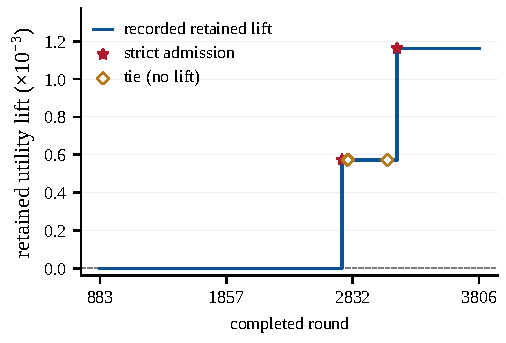
\includegraphics[width=\linewidth]{figures/fig_fw_retained_utility_lift.pdf}
  \caption{\textbf{Retained utility rises in two steps above the round-882 incumbent.}
  All \num{2924} completed records in rounds 883--3806, captured at 17:33 UTC
  on 2 November 2026. Each step is
  $\Delta u_r=u_{\mathrm{best},r}-u_{\mathrm{best},882}$, using the same
  recorded round-882 incumbent throughout. Vertical tick values denote
  $10^{-3}$ logged utility units. Stars mark two accepted strict gains;
  hollow diamonds mark two accepted ties, which add no lift. The other
  \num{2920} decisions are rejections. Classification uses unrounded logged
  values. Repeated development reuse prevents treating this curve as an
  independent learning or proposal-quality result. Scope: \cref{sec:method-status}.}
  \label{fig:fw-retained-utility-lift}
\end{figure}

\subsection{Recorded admission frequencies}\label{app:admission-outcomes}

\Cref{fig:fw-admission-outcomes} retains every completed decision in its
cumulative denominator. Admission includes exact ties; a separate line
counts strict utility gains. Both are descriptive frequencies on reused
development contexts (\cref{sec:method-status}).

\subsection{Current adapter admission decisions}\label{app:live-adapter-decisions}

Complete entries in the summary, adapter-admission and \mbox{per-round}
journals supply the scalar decisions in \cref{fig:fw-live-adapter-decisions}.

\begin{figure}[!tb]
  \centering
  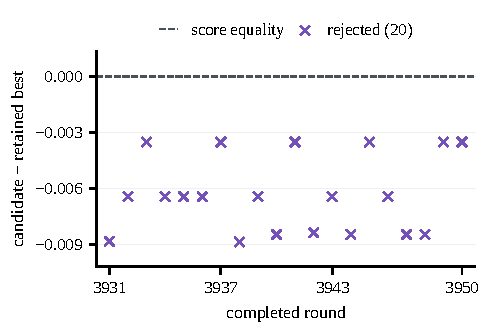
\includegraphics[width=\linewidth]{figures/fig_fw_live_adapter_decisions.pdf}
  \caption{\textbf{All 20 candidates in the window are rejected.}
  Rounds 3931--3950, captured at 23:00 UTC on 2 November 2026.
  Each point is candidate validation-pool utility minus the pre-decision retained best;
  zero denotes equality. Markers show logged admission decisions, with
  all 20 candidates rejected. Retained-best utility remains \num{1.1389572}.
  This adaptive window does not measure \mbox{independent}
  first-proposal or serving performance. Scope: \cref{sec:method-status}.}
  \label{fig:fw-live-adapter-decisions}
\end{figure}

The full admission record follows retained utility from round 775
(\cref{fig:fw-retained-best-plateau}).
\Cref{fig:fw-pool-insertions} separately counts pool insertions and adapter
rejections in its stated historical window.

\begin{figure}[!tb]
  \centering
  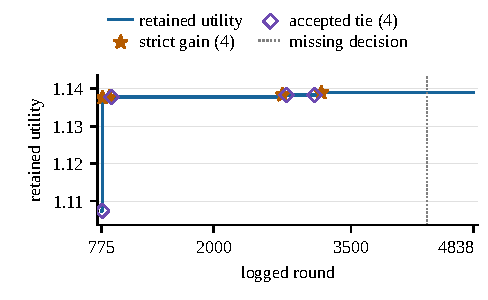
\includegraphics[width=\linewidth]{figures/fig_fw_retained_best_plateau.pdf}
  \caption{\textbf{Four strict gains and four ties mark the retained-utility record.}
  All \num{4063} logged adapter decisions in rounds 775--4838, captured
  at 04:56 UTC on 4 November 2026. Blue: post-decision retained utility;
  stars: strict gains; diamonds: accepted ties. Round 4331 is absent;
  the curve does not bridge it. Every recorded score is used, without a
  cumulative maximum or smoothing. This adaptive development record is not
  independent first-proposal or learning-gain evidence. Scope: \cref{sec:method-status}.}
  \label{fig:fw-retained-best-plateau}
\end{figure}

\begin{figure}[!tb]
  \centering
  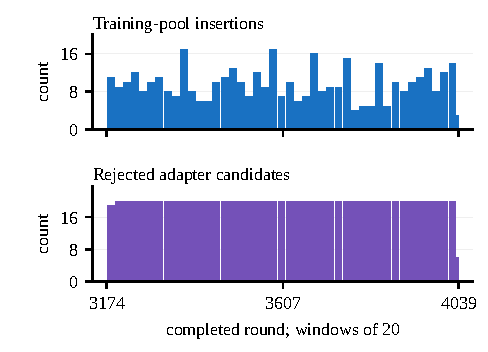
\includegraphics[width=\linewidth]{figures/fig_fw_pool_insertions.pdf}
  \caption{\textbf{Pool insertions and adapter rejections count different events.}
  Rounds 3174--4039, from complete journal prefixes captured on
  3 November 2026. Top: 421 logged automatic training-pool insertion
  events. Bottom: 865 rejected adapter candidates out of 866 decisions.
  Bars sum 20 consecutive completed rounds; the final bar covers six.
  Program-level insertions (events per window) and adapter rejections
  (decisions per window) have different units.
  These adaptive counts do not measure independent first-proposal
  \mbox{or learning gains. Scope: \cref{sec:method-status}.}}
  \label{fig:fw-pool-insertions}
\end{figure}

\subsection{Aligned event counters}\label{app:event-counters}

\Cref{fig:event-counters} aligns two committed histories sharing logged round
identifiers. The consecutive insertion records bracket the full admission
window; rounds without a recorded insertion are retained as zero counts. An insertion does not imply an adapter admission.

\begin{figure}[tb]
  \centering
  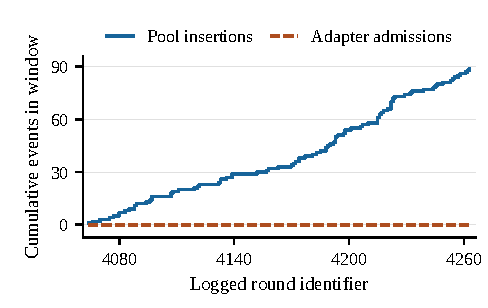
\includegraphics[width=\linewidth]{figures/fig_event_counters.pdf}
  \caption{\textbf{Pool insertions accumulate without adapter admission.}
  All 200 admission decisions in rounds 4064--4263, aligned with every
  program/context insertion in the committed history over those round
  identifiers. Blue: cumulative pool insertions; orange: cumulative adapter
  admissions. The window contains 89 insertions and zero adapter
  admissions. Each count starts at the window boundary and includes all
  events through the displayed round. These are distinct engineering-event
  counts, not independent proposal outcomes or evidence of learning gain.
  Scope: \cref{sec:method-status}.}
  \label{fig:event-counters}
\end{figure}

% No \FloatBarrier here: it ejected a column under the last lines of D.10 (a 30-line hole on that page),
% and the D.1-D.10 figures already reach their pages by [tbp] placement.
\subsection{Insertion frequency in fixed round windows}\label{app:pool-insertion-windows}

\Cref{fig:pool-insertion-windows} partitions the insertion history in
\cref{app:event-counters} into ten consecutive, nonoverlapping windows of
20 logged rounds. Every round contributes to exactly one window; the
first window starts at the committed admission history's first round.
The denominator is logged rounds, not candidate attempts or elapsed time.

\begin{figure}[tb]
  \centering
  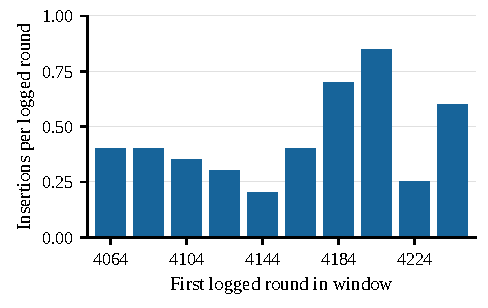
\includegraphics[width=\linewidth]{figures/fig_pool_insertion_windows.pdf}
  \caption{\textbf{Pool-insertion frequency varies across fixed round windows.}
  All ten nonoverlapping 20-round windows in rounds 4064--4263 of the
  committed history. Each bar is its exact insertion count divided by 20;
  the horizontal coordinate is the first round in that window. All 89
  insertions are retained. These engineering-event rates do not measure
  per-attempt success, wall-clock throughput or independent learning gain.
  Scope: \cref{sec:method-status}.}
  \label{fig:pool-insertion-windows}
\end{figure}

\subsection{Program-incumbent promotion margins}\label{app:program-promotion-margins}

\Cref{fig:program-promotion-margins} extends the retained program-promotion
record to the run's last event. Each margin compares programs in one
context; the admitted-event journal supplies no proposal-attempt denominator.

\begin{figure}[!tb]
  \centering
  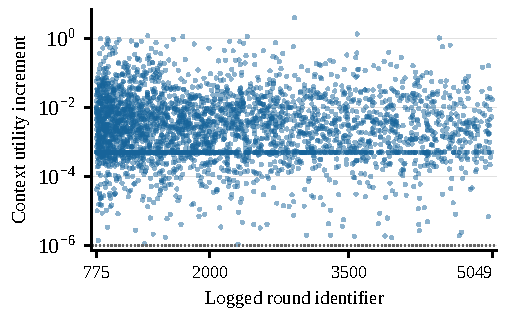
\includegraphics[width=\linewidth]{figures/fig_program_promotion_margins.pdf}
  \caption{\textbf{Program-incumbent promotions have unequal utility margins.}
  All \num{3529} ordinary promotion records in rounds 775--5049; the
  last is at round 5047 (11:13 UTC, 4 November 2026). Each point
  subtracts old from new logged utility in its own training context;
  larger is better. Pre-775 warm-up and historical admissions are
  excluded. Logarithmic axis; dotted line: the $10^{-6}$ admission margin.
  Admission requires positive increments. These cannot be summed
  across contexts or interpreted as proposal success, adapter improvement
  or writer learning. Scope: \cref{sec:method-status}.}
  \label{fig:program-promotion-margins}
\end{figure}

% Program-incumbent events and operating clocks.
\subsection{Earlier utility aggregates and operating measurements}\label{app:earlier-operating-records}

The earlier detailed summaries in \cref{fig:fw-trainval} cover only 25 rounds. In that subset,
training utility exceeds validation utility by 0.282--0.290
(\cref{fig:fw-trainval}). This is a difference between reported aggregates
on separate training and validation contexts; it does not isolate a cause
or establish behavior in the missing summaries. The late validation plateau
is evidence to explain, rather than proof of useful transfer. Encoder
integrity and parameter updates require their own receipts; the plotted
utility tables do not establish either.

\begin{figure*}[!t]
  \setlength{\abovecaptionskip}{4pt}
  \centering
  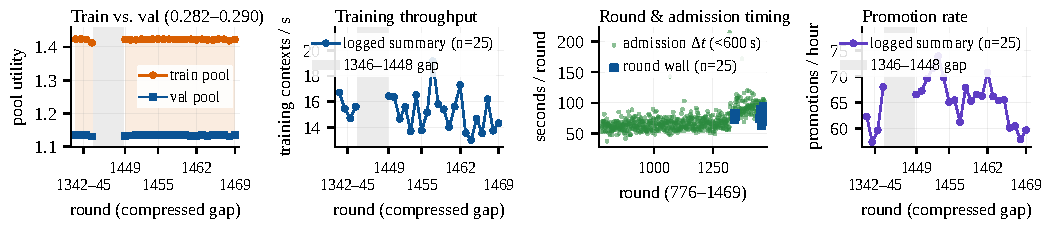
\includegraphics[width=\linewidth,height=1.50in,keepaspectratio]{figures/fig_fw_telemetry.pdf}
  \caption{\textbf{Train--validation aggregates and operating measurements from earlier retained windows.}
  First, second and fourth panels: 25 retained summaries spanning rounds 1342--1345 and 1449--1469
  (rounds 1346--1448 were not retained), showing train versus validation pool utility (gap 0.282--0.290),
  distinct training contexts per completed-round second and strict training-program promotions per hour
  over up to 20 completed rounds including qualification waits. Third panel: consecutive admission-timestamp
  intervals: all 695 admission rows (775--1469) carry timestamps, giving 694 consecutive pairs.
  The panel plots the 692 positive differences below 600\,s (green), excluding two longer pauses,
  alongside the 25 measured round wall times (blue squares).
  Scope: \cref{sec:method-status}.}
  \label{fig:fw-telemetry}
  \label{fig:fw-trainval}
\end{figure*}

\paragraph{Retained operating windows.}
In the five earlier 20-round program-event slices, rounds 2005--2024 record 15
events (\cref{fig:fw-recent-development}), rounds 2082--2101 record 10
(\cref{fig:fw-followup-development}), rounds 2343--2362 record 22
(\cref{fig:fw-later-development}), rounds 2508--2527 record 15
(\cref{fig:fw-subsequent-window}), and rounds 2644--2663 record 21
(\cref{fig:fw-program-promotions}). Each slice records zero adapter admissions.
The later 20-round throughput slice, 2696--2715, also records none; it
reports contexts and wall time rather than a program-event total.
Completed-time, event-distribution and rate summaries appear in
\cref{app:development-time,app:event-counts,app:subsequent-rates,app:promotions-per-hour,app:round-throughput}.
Scope and clock definitions follow \cref{sec:method-status}.

\subsection{Completed-round development trajectories}\label{app:development-time}\label{app:promotions-per-hour}

\Cref{fig:fw-completed-time} pairs four retained windows.
The separate 2644--2663 trajectory appears once in
\cref{fig:fw-promotions-per-hour}: per-round and
rolling program-event rates alongside candidate and recorded-best utility.
Whole-window rates are compared in \cref{fig:fw-latest-event-rates}.

\begin{figure*}[!t]
  \setlength{\abovecaptionskip}{4pt}
  \centering
  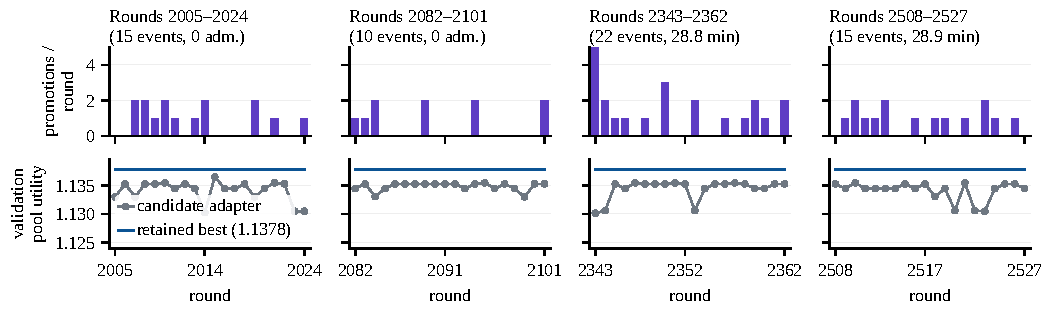
\includegraphics[width=\linewidth,height=2.10in,keepaspectratio]{figures/fig_fw_recent_development.pdf}
  \caption{\textbf{Four 20-round windows record program promotions with zero adapter admissions.}
  Columns show four separate 20-round summary windows: rounds 2005--2024 (15 events),
  2082--2101 (10 events), 2343--2362 (22 events over 28.8\,min of completed-round wall time)
  and 2508--2527 (15 events over 28.9\,min). Top row: strict training-program incumbent
  promotions per completed round. Bottom row: candidate adapter validation pool utility (grey)
  and the post-decision recorded best (blue, \num{1.1378} from round 882). Every window records zero
  adapter admissions. The separate 2644--2663 window is shown once in
  \cref{fig:fw-promotions-per-hour}. Scope: \cref{sec:method-status}.}
  \label{fig:fw-completed-time}
  \label{fig:fw-recent-development}
  \label{fig:fw-followup-development}
  \label{fig:fw-later-development}
  \label{fig:fw-subsequent-window}
  \label{fig:fw-subsequent-utility}
  \label{fig:fw-subsequent-rates}
\end{figure*}

\subsection{A subsequent development window}\label{app:subsequent-window}\label{app:subsequent-utility}\label{app:subsequent-rates}

The fourth column of \cref{fig:fw-completed-time} pairs per-round
program-event counts with candidate and recorded-best utility for rounds
2508--2527. Its 20 summaries contain 15 strict program-incumbent events and
zero adapter admissions. \Cref{app:earlier-operating-records} lists the separate window counts.

The utility panel uses its original scale. The retained
best is 1.1378 (recorded identity: round 882); that identity is not the first
round of strict gain.

These summaries total \num{1731.45}\,s. Dividing total counts by total logged time gives 41.58 completed
rounds per hour and 31.19 events per hour; these are not averages of per-round rates.
\Cref{fig:fw-latest-event-rates} places the event rate and mean round duration
alongside the other timed windows. The underlying per-round times remain
in the retained window record; they are not plotted again here.

\subsection{Program-event rate and round duration across windows}\label{app:latest-event-rates}

\Cref{fig:fw-latest-event-rates} consolidates four retained windows with
raw event counts and wall durations and a fresh matched 20-round capture.
Each rate divides that window's total events by its total completed-round
wall time; each mean duration divides the same time by 20. Sources lacking
raw duration, or lacking 20 consecutive rounds, are excluded rather than
imputed. The last of those five windows, rounds 3001--3020, records 12 program events
over \num{1809.50}\,s and no adapter admissions. Its summary event counts
match the promotion journal. Scope and window-separation rules follow
\cref{sec:method-status}.

\begin{figure*}[!t]
  \setlength{\abovecaptionskip}{4pt}
  \centering
  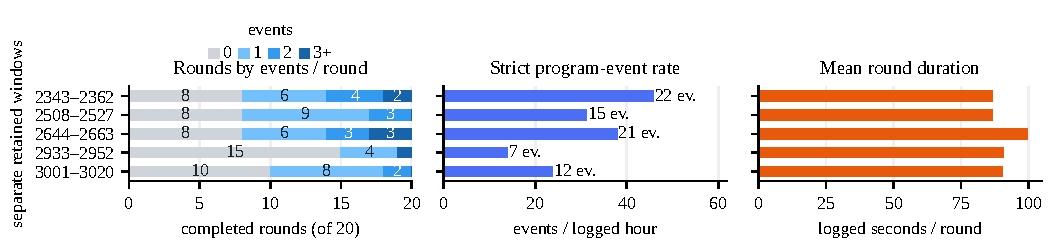
\includegraphics[width=\linewidth,height=1.65in,keepaspectratio]{figures/fig_fw_latest_event_rates.pdf}
  \caption{\textbf{Event distributions, program-event rates and round durations across retained 20-round windows.}
  Each row is a separate capture of 20 consecutive completed rounds with logged wall times.
  Left: completed rounds grouped by 0, 1, 2 or 3+ strict training-program incumbent events.
  Center: strict training-program incumbent events divided by total logged round time (events per hour), with total
  window event counts annotated. Right: mean completed-round duration (seconds) over the 20 rounds, including
  all within-round work and waits. Windows are displayed separately; program events are distinct
  from adapter admissions. Scope: \cref{sec:method-status}.}
  \label{fig:fw-event-distribution}
  \label{fig:fw-latest-event-rates}
\end{figure*}

\subsection{A full-run wall-time record}\label{app:latest-round-clock}

Logged round durations span the admission period
(\cref{fig:fw-latest-round-clock}); these operating clocks are separate from
the admission counts in \cref{tab:admission-ledger}.
Pricing a game-day proposal still requires \mbox{the full attempt} ledger (\cref{sub:price-run}).

% Graphic left, caption right (as Figure 40): a column-width graphic alone left the other column empty under the full-width figures.
\begin{figure*}[!t]
  \setlength{\abovecaptionskip}{4pt}
  \begin{minipage}[t]{\dimexpr.5\textwidth-.5\columnsep\relax}
  \vspace{0pt}
  \centering
  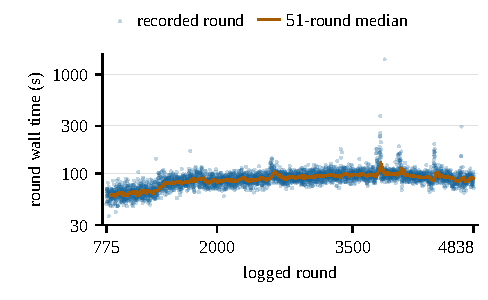
\includegraphics[width=\linewidth]{figures/fig_fw_latest_round_clock.pdf}
  \end{minipage}\hfill
  \begin{minipage}[t]{\dimexpr.5\textwidth-.5\columnsep\relax}
  \vspace{0pt}
  \caption{\textbf{Recorded round durations vary across the full admission period.}
  All \num{4064} retained wall-time records in rounds 775--4838, captured at
  04:58 UTC on 4 November 2026. Each point is a logged round's wall seconds;
  the line is the trailing 51-round median, starting with the 51st record.
  The vertical axis is logarithmic; no raw duration is filtered.
  These clocks include timed in-round work and waits, not inter-round gaps
  or single-proposal latency. Scope: \cref{sec:method-status}.}
  \label{fig:fw-latest-round-clock}
  \end{minipage}
\end{figure*}


\subsection{Throughput and program-incumbent diagnostics}\label{app:round-throughput}\label{app:program-gain-distribution}\label{app:current-program-clock}

% Defined before the text, so the figure can head the page after D.18 opens.
\begin{figure*}[!t]
  \setlength{\abovecaptionskip}{4pt}
  \begin{minipage}[t]{\dimexpr.5\textwidth-.5\columnsep\relax}
  \vspace{0pt}
  \centering
  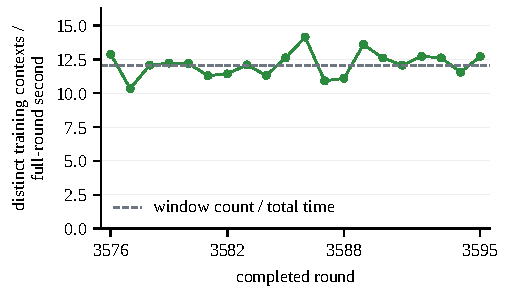
\includegraphics[width=\linewidth]{figures/fig_fw_live_round_throughput.pdf}
  \caption{\textbf{Completed-round throughput varies across rounds 3576--3595.}
  Twenty consecutive rounds, 3576--3595, captured at 09:54 UTC on
  2 November 2026. Each point divides \num{1219} distinct training contexts by
  that round's full wall time (contexts per second), including all work and
  waits. The dashed line divides the window's summed counts by summed time.
  Repeated contexts across rounds are not independent tasks; this is an
  operating observation, not \mbox{deployment} throughput.
  Scope: \cref{sec:method-status}.}
  \label{fig:fw-live-round-throughput}
  \end{minipage}\hfill
  \begin{minipage}[t]{\dimexpr.5\textwidth-.5\columnsep\relax}
  \vspace{0pt}
  \centering
  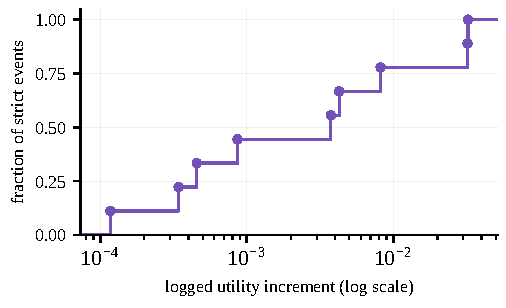
\includegraphics[width=\linewidth,height=2.05in,keepaspectratio]{figures/fig_fw_program_gain_distribution.pdf}
  \caption{\textbf{Nine strict program events occur across rounds 3656--3675.}
  Rounds 3656--3675, captured at 12:25 UTC on 2 November 2026.
  The empirical cumulative distribution gives each of the nine strict events
  equal weight; the horizontal axis is logarithmic. An increment is the
  journaled new utility minus its previous incumbent utility, computed
  from unrounded values. All 20 completed rounds are checked against the
  journal; 13 have no event and contribute no zero-gain observation.
  The window records zero adapter admissions. Event-level confidence
  intervals are unavailable; the curve is \mbox{descriptive,} without uncertainty
  bands. Scope: \cref{sec:method-status}.}
  \label{fig:fw-program-gain-distribution}
  \end{minipage}
  \par\medskip
  \begin{minipage}[t]{\dimexpr.5\textwidth-.5\columnsep\relax}
  \vspace{0pt}
  \centering
  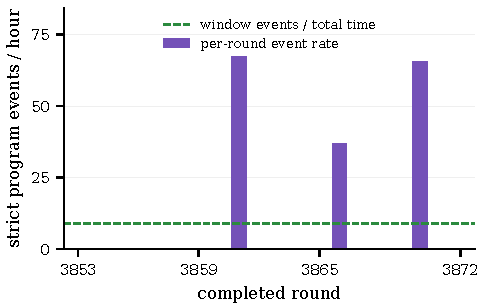
\includegraphics[width=\linewidth,height=2.05in,keepaspectratio]{figures/fig_fw_current_program_clock.pdf}
  \end{minipage}\hfill
  \begin{minipage}[t]{\dimexpr.5\textwidth-.5\columnsep\relax}
  \vspace{0pt}
  \caption{\textbf{Twelve strict program events occur across rounds 3931--3950.}
  Rounds 3931--3950, captured at 23:00 UTC on 2 November 2026.
  Bars divide each round's event count by its full wall time (events per hour);
  the dashed line divides the 12 events by the total
  \num{1987.27}\,s (21.74 events per hour). All 20 rounds are retained,
  including 10 with no event. The window records zero adapter admissions
  and no retained-utility gain; these program events do not measure
  independent first-proposal or game-day serving \mbox{performance. Scope: \cref{sec:method-status}.}}
  \label{fig:fw-current-program-clock}
  \end{minipage}
\end{figure*}

The 20-round 2696--2715 slice in \cref{fig:fw-round-throughput}, captured
at 06:54 UTC on 1 November 2026, has no adapter admission. Summary and
admission journals agree on candidate utility, recorded best, acceptance
and best-round identity. \Cref{fig:fw-live-round-throughput} adds a later
capture. Completed-round throughput divides distinct training contexts
by full round time; it differs from presentations per training second and
does not count \mbox{distinct tasks across} rounds.

The increments in \cref{fig:fw-program-gain-distribution} are logged
utility changes, not Elo changes or independent performance estimates.
The event counts in \cref{fig:fw-current-program-clock} are checked
against the promotion journal.


% Historical search diagnostics are distinct from the live admission record.
\subsection{Historical GP search diagnostics}\label{app:historical-search}

Historical GP target scores provide a separate view in the first panel of
\cref{fig:fw-target-progress}. The 159 repeated dataset/cut/arm groups cover
55 distinct dataset/cut pairs; the 64 groups with lower final scores cover
23 pairs. Shared incumbent and teacher seeds make the arms dependent.
Scope: \cref{sec:method-status}.

The remaining three panels of \cref{fig:fw-target-history} follow one
historical dataset/cut, chosen after inspection for the largest
policy-seeded relative improvement in the preceding comparison set. Every
reported generation is shown, without applying a cumulative minimum. All
three arms finish at the same value; the policy-seeded arm first records it
one generation after the controls. Shared seeds prevent treating their
matching outcomes as independent discoveries.

\begin{figure*}[!t]
  \setlength{\abovecaptionskip}{4pt}
  \centering
  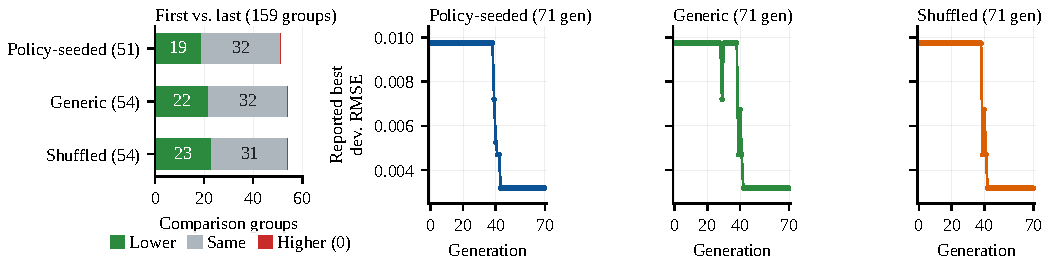
\includegraphics[width=\linewidth,height=1.50in,keepaspectratio]{figures/fig_fw_target_history.pdf}
  \caption{\textbf{Historical GP target progress and post-hoc 71-generation trajectories.}
  First panel: first-to-last reported best development RMSE across all 159 repeated comparison
  groups (55 distinct dataset/cut pairs) at \num{1000} evaluations per search, grouped by search arm.
  Second through fourth panels: all 71 generations per arm for one historical dataset/cut selected
  post hoc for the largest policy-seeded relative improvement. RMSE is in historical evaluator units
  (lower is better). The arms shared incumbent and teacher seeds, and elapsed time varied; these
  development records do not establish independent discoveries or a learned-policy advantage.}
  \label{fig:fw-target-progress}
  \label{fig:fw-target-history}
\end{figure*}


\begin{figure*}[!t]
  \setlength{\abovecaptionskip}{4pt}
  \centering
  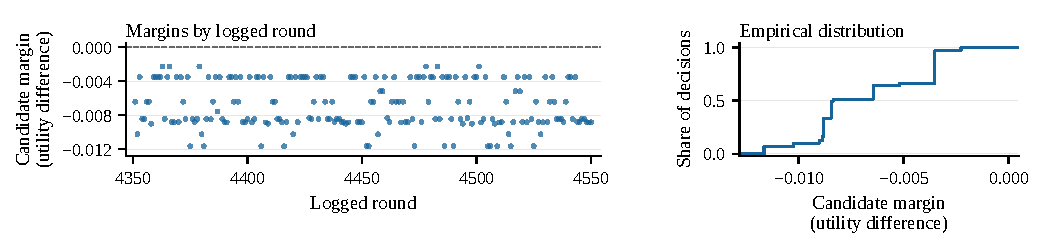
\includegraphics[width=\linewidth]{figures/fig_candidate_margin_window.pdf}
  \caption{\textbf{Adapter candidates remain below prior retained utility in the fixed window.}
  All 200 recorded admission decisions in rounds 4351--4550, captured at
  23:20 UTC on 3 November 2026. Left: candidate utility minus the explicit
  pre-decision retained utility; negative values mean lower candidate utility.
  Right: the empirical cumulative distribution of the same 200 signed margins,
  weighting each decision equally. The journal records zero admissions.
  No smoothing, imputation or cumulative minimum is applied.
  These adaptive development-pool observations do not establish an independent
  learning gain. Scope: \cref{sec:method-status}.}
  \label{fig:candidate-margin-window}
\end{figure*}

\subsection{A later candidate-margin window}\label{app:candidate-margin-window}

\Cref{fig:candidate-margin-window} follows the earlier pre-decision margin
view in \cref{fig:fw-admission-margins} with a fixed later window.
Its empirical distribution counts decisions, not independent tasks or
programs; the common telemetry scope applies (\cref{sec:method-status}).


\begin{figure}[!t]
  \setlength{\abovecaptionskip}{4pt}
  \centering
  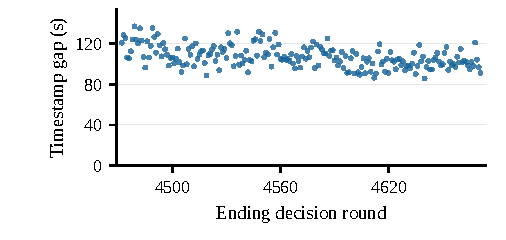
\includegraphics[width=\linewidth]{figures/fig_decision_cadence.pdf}
  \caption{\textbf{Recent adapter decisions arrive at varying intervals.}
  All 200 timestamp gaps between the latest 201 complete journal records,
  rounds 4471--4671, captured at 23:57 UTC on 3 November 2026.
  Each point subtracts the previous recorded timestamp from the current one
  and is keyed to the ending decision round. Both endpoint source lines
  and hashes are retained. These intervals include work, qualification waits
  and recording gaps; they measure record cadence, not compute time,
  single-proposal latency or learning. Scope: \cref{sec:method-status}.}
  \label{fig:decision-cadence}
\end{figure}
\FlushFloatsInPlace% keep the final cadence figure ahead of its subsection and References

\subsection{A recent decision-cadence snapshot}\label{app:decision-cadence}

\Cref{fig:decision-cadence} complements the separate utility-margin
snapshot in \cref{fig:candidate-margin-window}; the two windows do not
support a joint quality--cost comparison.


\subsection{Candidate parameter displacement}\label{app:parameter-displacement}

\href{eurekazero_supplement.pdf#supp-parameter-displacement}{Supplementary Figure~S1} retains the recorded
candidate displacement before admission, including perturbation and
optimization. It establishes no retained learning gain.


\subsection{Candidate gradient magnitudes}\label{app:gradient-norms}

\Cref{fig:gradient-norms} adds a step-level diagnostic before admission;
retained learning remains a separate question.

\begin{figure}[!tb]
  \setlength{\abovecaptionskip}{4pt}
  \centering
  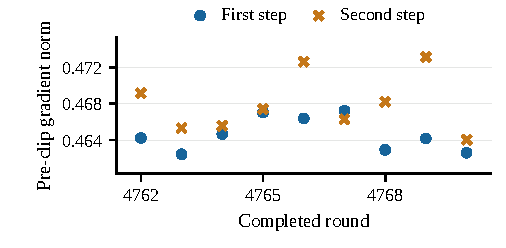
\includegraphics[width=\linewidth]{figures/fig_gradient_norms.pdf}
  \caption{\textbf{Candidate gradient norms vary across recorded steps.}
  All 9 complete retained summaries, rounds 4762--4770, captured at
  02:55 UTC on 4 November 2026. The 18 markers are logged pre-clip adapter
  gradient norms, two per candidate round. The steps use distinct training
  batches; their difference is not a matched loss reduction. No smoothing
  or filtering is applied. The window records zero admissions; these
  magnitudes establish no retained learning gain. Scope: \cref{sec:method-status}.}
  \label{fig:gradient-norms}
\end{figure}

\begin{figure*}[t]
  \setlength{\abovecaptionskip}{4pt}
  \centering
  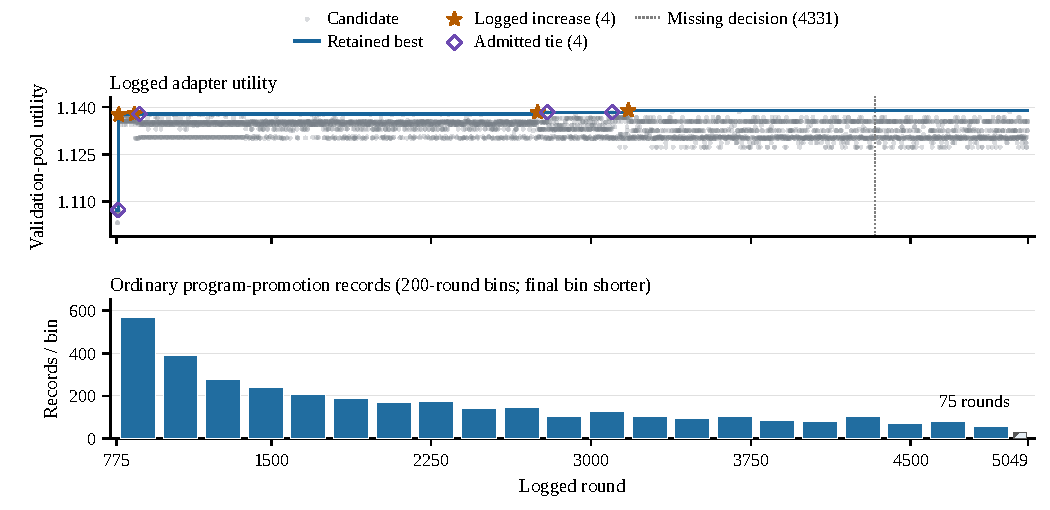
\includegraphics[width=\linewidth]{figures/fig_stopped_run_record.pdf}
  \caption{\textbf{Logged adapter utility and program-pool activity through round 5049.}
  Top: all \num{4274} recorded adapter decisions in rounds 775--5049,
  ending at 11:17 UTC on 4 November 2026. Grey: candidate validation-pool
  utility; blue: the logged retained best. Stars mark four logged increases,
  hollow diamonds four admitted ties. Round 4331 has no admission record;
  its dotted marker breaks the retained line. No smoothing or cumulative
  maximum is applied. Bottom: all \num{3529} ordinary training-program
  promotion records in the same round interval; the last event is at
  round 5047. Bars count fixed 200-round bins; the hatched final bin spans
  75 rounds. Historical admissions and earlier warm-up records are excluded.
  These conditional event counts are not proposal attempts or success rates,
  and the two journals have different admission rules. Reused validation
  contexts and unqualified runtime binding prevent interpreting this
  operating record as independent learning or a training effect.
  Scope: \cref{sec:method-status}.}
  \label{fig:stopped-run-record}
\end{figure*}


\subsection{Two admission records}\label{app:recent-discovery-retention}

\href[page=2]{eurekazero_supplement.pdf}{Supplementary Figure~S3} pairs program
promotions and adapter utility under distinct admission rules.


\subsection{Utility lift at each recorded decision}\label{app:recorded-decision-lift}

\href{eurekazero_supplement.pdf#supp-recorded-decision-lift}{Supplementary Figure~S4} gives candidate
and retained lift from the prior retained best; zero retained lift includes
rejection and accepted ties.


\subsection{Program-recording cadence}\label{app:program-record-cadence}

\href[page=2]{eurekazero_supplement.pdf}{Supplementary Figure~S5} shows
program-recording cadence.


\subsection{Operating record through round 5049}\label{app:stopped-run-record}

\Cref{fig:stopped-run-record} reaches the last adapter decision.
Supplementary Figures
\href{eurekazero_supplement.pdf#supp-program-complexity-changes}{S7} and
\href{eurekazero_supplement.pdf#supp-program-promotion-contexts}{S8}
report counted program-form changes and distinct recorded context
identifiers, respectively.
Program promotions and adapter admissions remain separate
(\cref{sec:method-status}).

